\documentclass[10pt]{beamer}

\usetheme{Warsaw}
%\addtobeamertemplate{navigation symbols}{}{%
%    \usebeamerfont{footline}%
%    \usebeamercolor[fg]{footline}%
%    \hspace{1em}%
%    \insertframenumber/\inserttotalframenumber
%}

\beamertemplatenavigationsymbolsempty

\setbeamertemplate{footline}
{
  \leavevmode%
  \hbox{%
  \begin{beamercolorbox}[wd=.333333\paperwidth,ht=2.25ex,dp=1ex,center]{author in head/foot}%
    \usebeamerfont{author in head/foot} \hyperlink{Patrolling games}{Locally-Observable Random Attackers}
  \end{beamercolorbox}%
  \begin{beamercolorbox}[wd=.333333\paperwidth,ht=2.25ex,dp=1ex,center]{title in head/foot}%
    \usebeamerfont{title in head/foot}\insertauthor
  \end{beamercolorbox}%
  \begin{beamercolorbox}[wd=.333333\paperwidth,ht=2.25ex,dp=1ex,right]{date in head/foot}%
    \usebeamerfont{date in head/foot}\insertshortdate{}\hspace*{2em}
    \insertframenumber{} / \inserttotalframenumber\hspace*{2ex} 
  \end{beamercolorbox}}%
  \vskip0pt%
}
\setbeamertemplate{headline}{}
\usefonttheme[onlymath]{serif}

\usepackage{color}
\usepackage{xcolor}
\usepackage{tikz}
\usepackage{amsmath}
\usepackage{amssymb}
\usepackage{amsthm}
\usepackage{amsfonts}
\usepackage{graphicx}
\usepackage{mathtools}
\usepackage{wrapfig}
\usepackage{multirow}
\usepackage{comment}
\usepackage{natbib}
\usepackage{appendix}
\usepackage[utf8]{inputenc}
\usepackage{floatrow}
\usepackage{newfloat}
\usepackage{subcaption}
\usepackage{bm}
\usepackage{hyperref}
\usepackage{tcolorbox}

\usetikzlibrary{calc}
\usetikzlibrary{fit}
\usetikzlibrary{decorations.shapes,shapes.misc,calc, positioning, hobby, backgrounds}

\tikzset{cross/.style={cross out, draw=black, minimum size=2*(#1-\pgflinewidth), inner sep=0pt, outer sep=0pt},
%default radius will be 1pt. 
cross/.default={1pt}}

\tikzset{decorate sep/.style 2 args=
{decorate,decoration={shape backgrounds,shape=circle,shape size=#1,shape sep=#2}}}

\DeclareFloatingEnvironment[fileext=los,
    listname={List of myFigures},
    name=Figure,
    placement=tbhp,
    within=section,]{myfigure}      



%\DeclarePairedDelimiter{\floor}{\lfloor}{\rightfloor}
%\DeclarePairedDelimiter{\ceil}{\lceil}{\rceil}

\newcommand{\halflength}{\ensuremath{\floor{\frac{m}{2}}}}
\newcommand{\floor}[1]{\left \lfloor #1 \right \rfloor}
\newcommand{\ceil}[1]{\left \lceil #1 \right \rceil}
\newcommand{\pospart}[1]{\left( #1 \right)_{+}}
\newcommand{\negpart}[1]{\left( #1 \right)_{-}}
\newcommand{\set}[2]{\left\{ #1 \, | \, #2 \right\}}

\newcommand{\oneline}[1]{\resizebox{\dimexpr\paperwidth - 3ex}{!}{#1}}

\DeclareMathOperator*{\argmin}{\arg\!\min}

%Text box tight style
\tcbset{mytight/.style={hbox,left=1mm,right=1mm,top=1mm,bottom=1mm,nobeforeafter}}

%\DeclareFloatingEnvironment[fileext=los,
 %   listname={List of Example Figures},
  %  name=Example Figure,
   % placement=tbhp,
    %within=section,]{examplefigure}

\author{Thomas Lowbridge and David Hodge}
\title{A Graph Patrol Problem with Locally-Observable Random Attackers}
%\setbeamercovered{transparent} 
%\setbeamertemplate{navigation symbols}{} 
%\logo{} 
\institute{University Of Nottingham,UK} 
\date{June 15, 2018} 
%\subject{} 
\begin{document}

\hypertarget{Patrolling games}{}
\begin{frame}
\titlepage
\end{frame}

%\begin{frame}
%\tableofcontents
%\end{frame}

\begin{frame}{Outline}

\begin{itemize}
\item Introduction to game
\begin{itemize}
\item Game setup
\item Markov Decision Process(MDP) formulation
\end{itemize}
\item Problem relaxation
\begin{itemize}
\item Multi-node relaxation
\item Total-rate relaxation
\item Lagrangain relaxation
\end{itemize}
\item Single node solution
\begin{itemize}
\item Developing an optimal policy
\item Developing a threshold policy
\item Fair costs
\end{itemize}
\item Indices and heuristics
\end{itemize}
\end{frame}


\begin{frame}{Game setup}
A Patrolling game with random attackers and local-observations, \textcolor{purple}{$G=G(Q,\bm{X},\bm{b},\bm{\lambda},\bm{c})$} is made of 5 major components.
\begin{itemize}
\item A \textcolor{purple}{Graph, $Q=(N,E)$}, made of nodes, $N$ ($|N|=n$), and a set of edges, $E$ and an adjacency matrix, \textcolor{purple}{$A$}.
\item A vector of \textcolor{purple}{attack time distributions, $\bm{X}=(X_{1},...,X_{n})$}.
\item A vector of \textcolor{purple}{observable capacities, $\bm{b}=(b_{1},...,b_{n})$}
\item A vector of \textcolor{purple}{poisson arrival rates, $\bm{\lambda}=(\lambda_{1},...,\lambda_{n})$}.
\item A vector of \textcolor{purple}{costs, $\bm{c}=(c_{1},...,c_{n})$}
\end{itemize}

\pause

The game is played over an infinite time horizon, $\mathcal{T}={0,1,....}$

A patroller's policy in the game is a walk (with waiting) on the graph,
$$W: \mathcal{T} \rightarrow N .$$
With the patroller moving instantaneously between nodes and attackers who arrive when the patroller is present waiting till the next time period to attack(who are observed as suspicious by the patroller).
\end{frame}

\begin{frame}{Markov Decision Process(MDP) formulation}
This game is a MDP with states $(\bm{s},\bm{v})$, where $s_{i}$ is the time since node $i$ was last chosen to be visited and $v_{i}$ is how many local-observations where observed when node $i$ was last visited. With state space $\Omega=\{(\bm{s},\bm{v}) | s_{i}=1,2,.... \, \text{and}  \, v_{i}=0,1,....,b_{i} \, \forall i=1,...,n  \}$.

\

The current node can be identified by $l(\bm{s})=\argmin_{i} \bm{s}$. The current node will have $s_{i}=1$. The available actions from any state is $\mathcal{A}(\bm{s})=\{j | A_{l(\bm{s}),j}=1 \}$.

\
 
A transition from a state,$(\bm{s},\bm{v})$, with a chosen action, $i$, is $\phi(\bm{s},\bm{v},i)=(\widetilde{\bm{s}},\widetilde{\bm{v}})$ where $\widetilde{s}$ has; $\widetilde{s}_{i}=1$ and $\widetilde{s}_{j}=s_{j}+1 \, \forall j \neq i$ and $\widetilde{v}$ has; $\widetilde{v}_{i} \sim TPo(\lambda_{i})$ and  $\widetilde{v}_{j}=v_{i} \, \forall j \neq i$.

Where $TPo(\lambda,b)$ is the Poisson distribution truncated at the value $b$. I.e
\begin{align*}
P(TPo(\lambda,b)=\begin{cases}
P(Po(\lambda) \text{ if } i \neq b \\
P(Po(\lambda) \geq i) \text{ if } i=b \\
0 \text{ Otherwise}
\end{cases}
\end{align*}
Note. $TPo(\lambda,\infty)=Po(\lambda)$.

\end{frame}

\begin{frame}{Finiteness considerations}
To avoid certain problems, we would like to limit ourselves to a finite state space

\

Like in [Insert reference to paper], we will bound the attack times to create a finite state space, and define \textcolor{red}{$B_{j} \equiv \min \{ k | k \in \mathbb{Z}^{+} , P(X_{j} \leq k)=1 \}$}. We will also bound our observable capacities to finite integers \textcolor{red}{$b_{i} \in \mathbb{Z}^{+}_{0}$}.This restricts our state space to a finite size
$\Omega=\{(\bm{s},\bm{v}) | s_{i}=1,2,....,B_{i}+1 \, \text{and}  \, v_{i}=0,1,....,b_{i} \, \forall i=1,...,n  \}$.

\

Now however our transistions are limited and become $\phi(\bm{s},\bm{v},i)=(\widetilde{\bm{s}},\widetilde{\bm{v}})$ where $\widetilde{s}$ has; $\widetilde{s}_{i}=1$ and \textcolor{red}{$\widetilde{s}_{j}=\min \{s_{j}+1,B_{j}+1 \} \forall j \neq i$} and $\widetilde{v}$ has; $\widetilde{v}_{i} \sim TPo(\lambda_{i},b_{i})$ and  $\widetilde{v}_{j}=v_{i} \forall j \neq i$.

\end{frame}

\begin{frame}{Example of state space}

\begin{myfigure}[H]
\begin{center}
\resizebox{0.8\linewidth}{!}{
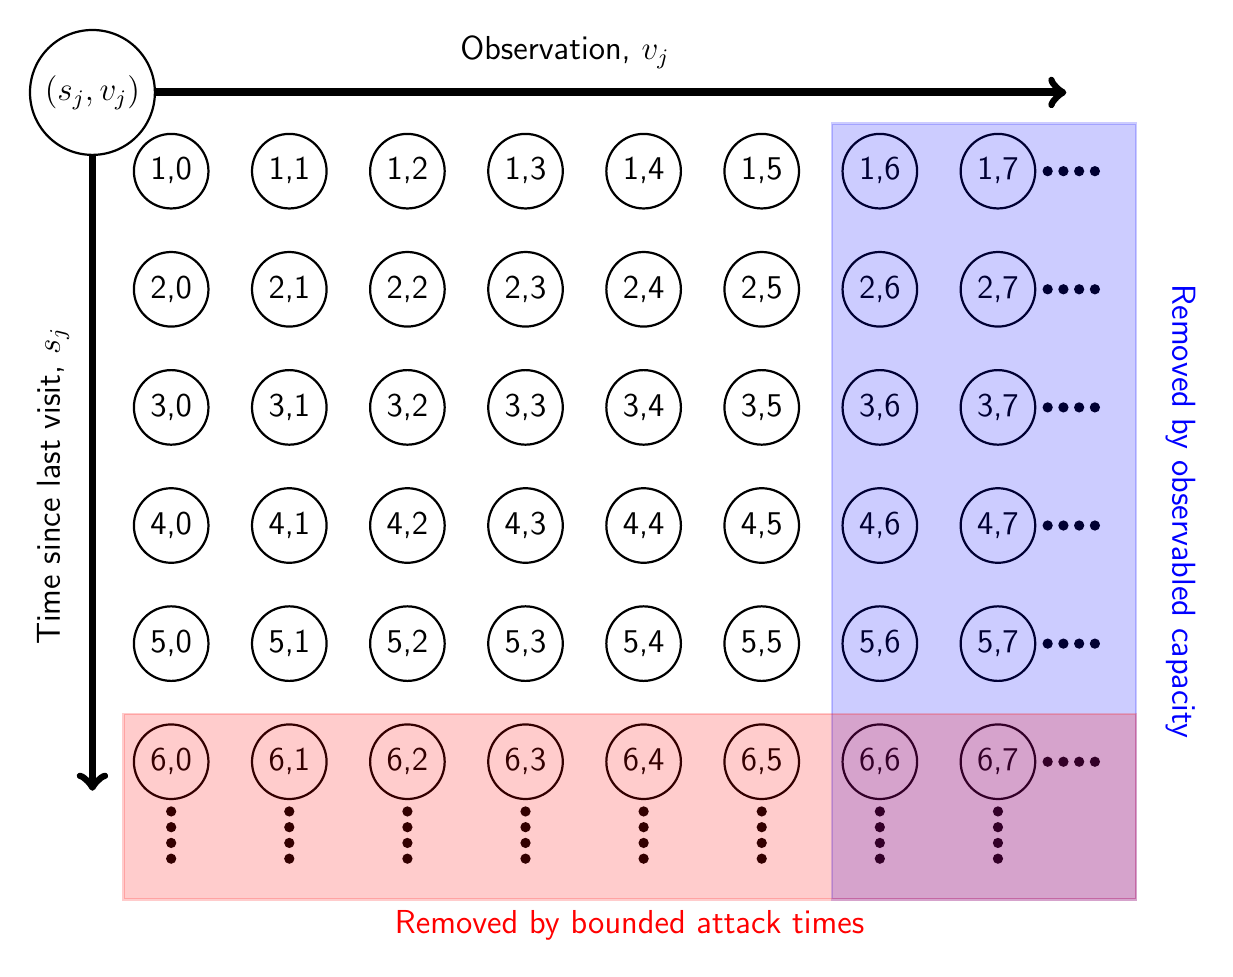
\begin{tikzpicture}[-,auto,node distance=1cm,
                    thick,main node/.style={circle,fill=white,draw,font=\sffamily\large,minimum size=0.5cm}]
 \foreach \x in {0,...,7}
    \foreach \y in {0,...,5} 
       {\pgfmathtruncatemacro{\label}{\x - 5 *  \y +21}
        \pgfmathtruncatemacro{\v}{\x}
        \pgfmathtruncatemacro{\s}{6-\y}
       \node [main node]  (\x\y) at (1.5*\x,1.5*\y) {\s,\v};} 

\node (XaxisLeft) [shift={(-0.5,1)}] at (05) {};
\node (XaxisRight) [shift={(1,1)}] at (75) {};

\node (YaxisBottom) [shift={(-1,-0.5)}] at (00) {};
\node (YaxisTop) [shift={(-1,1)}] at (05) {};

\draw[->,line width=1mm] (XaxisLeft)--(XaxisRight);
\draw[->,line width=1mm] (YaxisTop)--(YaxisBottom);

\node[font=\sffamily\large] (OLabel) [shift={(0.5,1.5)}] at (35) {Observation, $v_{j}$};
\node[font=\sffamily\large] (SLabel) [shift={(-1.5,0.5)}] at (02) {\rotatebox{90}{Time since last visit, $s_{j}$}};

\node[main node] (Example) [shift={(-1,1)}] at (05) {$(s_{j},v_{j})$};

\foreach \y in {0,...,5}
{\node (DottedStart\y) [shift={(0.5,0)}] at (7\y) {};
 \node (DottedEnd\y) [shift={(1.5,0)}] at (7\y) {};
 \draw[decorate sep={1mm}{2mm},fill] (DottedStart\y)--(DottedEnd\y);}
 
\foreach \x in {0,...,7}
{\node (\x DottedStart) [shift={(0,-0.5)}] at (\x0) {};
 \node (\x DottedEnd) [shift={(0,-1.5)}] at (\x0) {};
 \draw[decorate sep={1mm}{2mm},fill] (\x DottedStart)--(\x DottedEnd);
}

\node (Box1) [draw,thick,fit=(65) (60) (DottedEnd5) (DottedEnd0) (6DottedEnd) (7DottedEnd),fill,blue,opacity=0.2] {};

\node (Box2) [draw,thick,fit=(00) (70)(DottedEnd0) (0DottedEnd) (7DottedEnd),fill,red,opacity=0.2] {};

\node[font=\sffamily\large,color=blue] (Box1Text) [shift={(2.5,0)}] at (Box1) {\rotatebox{270}{Removed by observabled capacity}};

\node[font=\sffamily\large,color=red] (Box2Text) [shift={(0,-1.5)}] at (Box2) {Removed by bounded attack times};           

\end{tikzpicture}
}
\end{center}
\caption{State space diagram, with \textcolor{blue}{$b_{j}=5$} and \textcolor{red}{$B_{j}=4$} (e.g. $X_{j} \leq 3.7$)}
\end{myfigure}

\end{frame}

\begin{frame}{Markov Decision Process(MDP) formulation}
The cost at a node is zero if that node is chosen, otherwise it is the cost of arrivals finishing in the next time period, plus the cost of local-observations finishing in the next time period.
\
$$C_{j}(\bm{s},\bm{v},i)=\begin{cases}
\begin{split}
&c_{j} \lambda_{j} \int_{s_{j}-1}^{s_{j}} P(X_{j} \leq t) dt \\
&+ c_{j}v_{j}P(s_{j}-1 < X_{j} \leq s_{j}) \text{ if } j \neq i 
\end{split} \\
0 \text{ if } j=i \\
\end{cases}$$.

Due to the finiteness of the state space, we can just focus on stationary, deterministic policies, $\pi: \Omega \rightarrow \mathcal{A} \in \Pi$, instead of all walks, $\mathcal{W}$.
\end{frame}

\begin{frame}{Markov Decision Process(MDP) formulation}
The patroller wants to choose a policy such that the long-run average cost is minimized, that is find the minimum cost (and policy) defined by,

\begin{align*}
C^{\text{OPT}}(\bm{s}_{0},\bm{v}_{0}) \equiv \min\limits_{\pi \in \Pi} \sum\limits_{i=1}^{n} V_{i}(\pi,\bm{s}_{0},\bm{v}_{0})
\end{align*}

Where $V_{i}(\pi,\bm{s}_{0},\bm{v}_{0})$ is the long-run average cost incurred at node $i$ under the policy, $\pi$, starting from state, $(\bm{s}_{0},\bm{v}_{0})$ defined by ,

\begin{align*}
V_{i}(\pi,\bm{s}_{0},\bm{v}_{0}) \equiv \lim\limits_{N \rightarrow \infty} \frac{1}{N} \sum\limits_{k=0}^{N-1} C_{i}(\phi^{k}_{\pi}(\bm{s}_{0},\bm{v}_{0}),\pi(\phi^{k}_{\pi}(\bm{s}_{0},\bm{v}_{0})))
\end{align*}
Where $\phi^{k}_{\pi}(\bm{s}_{0},\bm{v}_{0})$ is the state after $k$ transitions starting from $(\bm{s}_{0},\bm{v}_{0})$ under the policy $\pi$.

\end{frame}

\begin{frame}{Problem Relaxation: Multiple Node}
We now relax the problem to that of a patroller who can visit multiple nodes in the next time period.

We will call this Problem the multiple-node(MN) problem. We extend the class of polcies to 

\begin{align*}
\Pi^{\text{MN}}= \{\pi \,  | \, \pi : \Omega \rightarrow \{\bm{\alpha} \, | \, \alpha_{i} \in \{0,1 \} \text{ for } i=1,...,n \}   \}
\end{align*}

Where $\alpha_{i}=1$ if the patroller will visit node $i$ in the next time period and $\alpha_{i}=0$ if the patroller will not visit node $i$ in the next time period.
Note. $\Pi \subset \Pi^{\text{MN}}$.
\end{frame}

\begin{frame}{Total-rate constraint}
\begin{definition}[Long-run visit rate]
Define the long-run rate of visits to node $i$, starting at $(\bm{s}_{0},\bm{v}_{0})$ under policy $\pi$ by
\begin{align*}
\mu_{i}(\pi,\bm{s}_{0},\bm{v}_{0})=\lim\limits_{N \rightarrow \infty} \frac{1}{N} \sum\limits_{k=0}^{N-1} \alpha_{\phi_{\pi}^{k}(\bm{s}_{0},\bm{v}_{0}),i}
\end{align*}
\end{definition}

We now impose the \textcolor{purple}{total-rate} constraint, that is the long-run overall visit rate to all nodes is no greater than 1. and restrict the MN problem by this to get the total-rate(TR) problem and its class of policies

\begin{align*}
\Pi^{\text{TR}}=\left\{ \pi \in \Pi^{\text{MN}} \, \bigg| \, \sum\limits_{i=1}^{n} \mu_{i}(\pi,\bm{s}_{0},\bm{v}_{0}) \leq 1 \quad \forall (\bm{s}_{0},\bm{v}_{0}) \in \Omega \right\}
\end{align*}

Again $\Pi \subset \Pi^{\text{TR}}$.
\end{frame}

\begin{frame}{Lagrangian relaxation}
We now relax the problem again by incorporating the total rate constraint into the objective function, with a Lagrange multiplier, $\omega \geq 0$. This forms

\begin{align*}
C(\omega)&=\min_{\pi \in \Pi^{\text{MN}}} \left\{ \sum\limits_{i=1}^{n} V_{i}(\pi) + \omega \left( \sum\limits_{i=0}^{n} \mu_{i}(\pi) -1 \right) \right\} \\
&=\min_{\pi \in \Pi^{\text{MN}}} \sum\limits_{i=1}^{n} (V_{i}(\pi)+\omega \mu_{i}(\pi)) - \omega
\end{align*}

By incorporating the total-rate constraint as a Lagrange multiplier we can drop the constraint, so that the patroller can choose to visit any number of nodes in each time period (each costing $\omega$).
\end{frame}

\begin{frame}{Linking reduced problems}
We have that for any $\omega \geq 0$

\begin{align*}
C^{\text{TR}}=\min_{\pi \in \Pi^{\text{TR}}} \sum\limits_{i=1}^{n} V_{i}(\pi) &\geq \min_{\pi \in \Pi^{\text{TR}}} \left\{ \sum\limits_{i=1}^{n} V_{i}(\pi) + \omega \left( \sum\limits_{i=0}^{n} \mu_{i}(\pi) -1 \right) \right\} \\
&\geq \min_{\pi \in \Pi^{\text{MN}}} \left\{ \sum\limits_{i=1}^{n} V_{i}(\pi) + \omega \left( \sum\limits_{i=0}^{n} \mu_{i}(\pi) -1 \right) \right\}=C(\omega)
\end{align*}

The first inequality follows as the total-rate constraint is obeyed in $\Pi^{\text{TR}}$ and hence the $\omega \left( \sum\limits_{i=0}^{n} \mu_{i}(\pi) -1 \right) \leq 0$ and the second holds, as $\Pi^{\text{TR}} \subset \Pi^{\text{MN}}$.

\

Hence we have a string of inequalities $C^{\text{OPT}} \geq C^{\text{TR}} \geq C(\omega)$.
\end{frame}

\begin{frame}{Single node problem}
We now want to find $C(\omega)=\min\limits_{\pi \in \Pi^{\text{MN}}} \sum\limits_{i=1}^{n} (V_{i}(\pi)+\omega \mu_{i}(\pi)) - \omega$. This problem, as we are in the multi-node class, can be rewrote as

\begin{align*}
C(\omega)=\sum\limits_{i=1}^{n} \min\limits_{\pi \in \Pi^{\text{MN}}} (V_{i}(\pi)+\omega \mu_{i}(\pi)) - \omega
\end{align*}


That is for every node, $i$, try to minimize $V_{i}(\pi)+\omega \mu_{i}(\pi)$, where $\omega$ can be interpreted as the service charge for visiting the node.For now we drop the node subscript and just try to find the following,

\begin{align*}
\min_{\pi \in \Pi^{\text{MN}}} V(\pi) + \omega \mu(\pi)
\end{align*}

\end{frame}

\begin{frame}{Deterministic attack times}
Before looking at solving the single node problem, we will assume the attack times are deterministic, to make the cost function easier to handle.

When we use $X_{j}=x_{j}$ we get a cost function of.

For $s_{j} < B_{j}$
\begin{align*}
C_{j}(\bm{s},\bm{v},i)=0
\end{align*}

For $s_{j}=B_{j}$
\begin{align*}
C_{j}(\bm{s},\bm{v},i)= \begin{cases}
c_{j} \lambda_{j} R_{j} + c_{j} v_{j}  \text{ for } i \neq j \\ 
0 \text{ for } i=j \\
\end{cases}  
\end{align*}

For $s_{j}=B_{j}+1$
\begin{align*}
C_{j}(\bm{s},\bm{v},i)= \begin{cases}
c_{j} \lambda_{j} \text{ for } i \neq j \\
0 \text{ for } i=j \\
\end{cases}
\end{align*}

\end{frame}

\begin{frame}{Developing an optimal policy}
We know aim to develop and index on our state space, that is a fair price for visiting the node for a given state. We shall first show there is no fair price, $\omega$ for visiting in any state, $(s,v)$ with $s < B$.

From this position consider the policy $\pi_{k}$ which waits $k$ time periods and then renews and follows the optimal policy, $\sigma$, with $k=0,...,B-s$.

Using such a policy will get us that
\begin{equation}
V_{n}^{\pi_{k}}(x,v)=\omega + E[V_{n-k-1}^{\sigma}(\theta)]
\end{equation}

where $\theta$ is the state upon a visit (i.e it is the state $(1,V) \sim (1,TPo(\lambda))$.

Now we will pick policy $\pi_{k+1}$ over $\pi_{k}$ (or be indifferent) if

\begin{align*}
&\lim\limits_{n \rightarrow \infty} V_{n}^{\pi_{k}} (x,v) - V_{n}^{\pi_{k+1}}(x,v) \geq 0 \\
& \iff \lim\limits_{n \rightarrow \infty} E[V_{n-k}^{\sigma}(\theta) - V_{n-k-1}^{\sigma} (\theta)] \geq 0 \\
& \iff g \geq 0
\end{align*}
Where $g$ is the long-run average cost and so we know $g \geq 0$ hence we will always wait instead of renewing.
\end{frame}

\begin{frame}{Developing an optimal policy}
Now we will skip to the state $(B+1,v)$ and suggest again a policy $\pi_{k}$ which waits $k$ time periods before renewing and then follows some optimal policy, $\sigma$.

Using such a policy will get us
\begin{equation}
V_{n}^{\pi_{k}}(x,v)= \omega +c \lambda k + E[V_{n-k-1}^{\sigma}(\theta)]
\end{equation}

And again we will pick a policy $\pi_{k+1}$ over $\pi_{k}$ (or be indifferent) if

\begin{align*}
&\lim\limits_{n \rightarrow \infty} V_{n}^{\pi_{k}} (\floor{B}+2,0) - V_{n}^{\pi_{k+1}}(\floor{B}+2,0) \geq 0 \\
& \iff \lim\limits_{n \rightarrow \infty} -c \lambda + E[V_{n-k}^{\sigma}(\theta) - V_{n-k-1}^{\sigma}(\theta)] \geq 0 \\
& \iff g \geq c \lambda
\end{align*}

So hence if $g \geq c \lambda$ we will wait forever, as this has no dependence on $k$.

We will now argue that $g_{\text{max}}=c \lambda$, that is at worst the  long-run average cost is $c \lambda$. This can be seen by the strategy $\pi_{\text{neg}}$, a strategy which never renews no matter what state we are in. I.e the patroller neglects the node. As for large $n$ we just pay $c \lambda$ every time step. Hence in these states if we renew we will renew immediately.
\end{frame}

\begin{frame}{Developing an optimal policy}
Our neglecting strategy shows that $g \leq c \lambda$ and hence if we are in state $(B,v)$, we can decide to renew now or renew in one time period (at $(B+1,v)$) then follow the optimal, $\sigma$

we will choice to renew now over waiting if

\begin{align*}
&\lim\limits_{n \rightarrow \infty} V_{n}^{\pi_{1}} (B,v) - V_{n}^{\pi_{0}}(B,v) \geq 0 \\
& \iff \lim\limits_{n \rightarrow \infty} c \lambda R + vc + E[V_{n-1}^{\sigma}(B+1,0)] - (\omega + E[V_{n-1}^{\sigma}(\theta)]) \geq 0 \\
& \iff g \leq c (\lambda R +v) 
\end{align*}

So we renew now if $g \leq c (\lambda R +v)$, as we are guaranteed that $g \leq c \lambda$ we are clearly in this region if $ c (\lambda R +v) \leq c \lambda \iff v \leq \lambda (1-R)$. We also note that the bound is increasing in $v$ so if we will renew in $v$ we definitely renew in $v+1,v+2,...,b$.

\end{frame}

\begin{frame}{Developing a Threshold policy}

\begin{definition}[Threshold Policy]
Policy, $\pi_{\text{Th}}(v_{\text{crit}})$, is the policy which in states:
\begin{itemize}
\item $(s,v)$ , $s < B$ waits until $(B,v)$
\item $(B,v)$ renews now if $v \geq v_{\text{crit}}$ and waits until $(B+1,v)$ if $v < v_{\text{crit}}$
\item $(B+1,v)$ renews now.
\end{itemize}
\end{definition}

We notice that as we need $g \leq c(\lambda R + v)$ to renew now there is some maximum choice for this threshold, $v_{\text{max}} \equiv \max \{ v \in \{0,1,...,b \} \, | \, v \leq \lambda (1-R) \} $, so $v_{\text{crit}} \in \{0,1,...,v_{\text{max}}+1 \}$.

We get bounds on the long-run average cost
\begin{itemize}
\item $g \leq c \lambda R$ if $v_{\text{crit}}=0$.

\item $c \lambda R +c(k-1) < g \leq c \lambda R + kc$ if $v_{\text{crit}} \neq 0,v_{\text{max}}+1$

\item $c \lambda R + c v_{\text{max}} < g \leq c \lambda$ if $v_{\text{crit}}=v_{\text{max}}+1$
\end{itemize}

\end{frame}

\begin{frame}{Example of a threshold policy}
\begin{myfigure}[H]
\begin{center}
\resizebox{0.7\linewidth}{!}{
\begin{tikzpicture}[-,auto,node distance=1cm,
                    thick,main node/.style={circle,fill=white,draw,font=\sffamily\large,minimum size=0.5cm}]
 \foreach \x in {0,...,5}
    \foreach \y in {0,...,4} 
       {\pgfmathtruncatemacro{\label}{\x - 5 *  \y +21}
        \pgfmathtruncatemacro{\v}{\x}
        \pgfmathtruncatemacro{\s}{5-\y}
       \node [main node]  (\x\y) at (1.5*\x,1.5*\y) {\s,\v};}
       
       \node[main node] (Renewal) at (1.5*6,1.5*4) {$\theta$};

 \foreach \x in {0,...,1}
    \foreach \y in {2,...,5} 
       {\pgfmathtruncatemacro{\label}{\x - 5 *  \y +21}
        \pgfmathtruncatemacro{\v}{\x}
        \pgfmathtruncatemacro{\s}{5-\y}
        \pgfmathtruncatemacro{\nv}{\v}
        \pgfmathtruncatemacro{\ns}{5-\y+1}
       \draw[->] (\nv\ns)--(\v\s);}
       
  \foreach \x in {2,...,5}
    \foreach \y in {2,...,4} 
       {\pgfmathtruncatemacro{\label}{\x - 5 *  \y +21}
        \pgfmathtruncatemacro{\v}{\x}
        \pgfmathtruncatemacro{\s}{5-\y}
        \pgfmathtruncatemacro{\nv}{\v}
        \pgfmathtruncatemacro{\ns}{5-\y+1}
       \draw[->] (\nv\ns)--(\v\s);}
       
    \foreach \x in {2,...,5}
       {\draw[-] (\x1) to (1.5*\x,1.5 *0.4);}
                 
        \draw[-] (1.5*2,1.5*0.4) to (1.5*6,1.5*0.4);
        \draw[->] (1.5*6,1.5*0.4) to (Renewal);                          

    \foreach \x in {0,...,5}
       {\draw[-] (\x0) to (1.5*\x,-1.5*0.6);}
       
       \draw[-] (1.5*0,-1.5*0.6) to (1.5*6,-1.5*0.6);                                            
       \draw[-] (1.5*6,-1.5*0.6) to (1.5*6,1.5*0.4);                                 
       
    \foreach \x in {0,...,5}
    { 
     \draw[->,bend right,dashed] (Renewal) to (\x4);    
    }   
        

\node (XaxisLeft) [shift={(-0.5,0.5)}] at (05) {};
\node (XaxisRight) [shift={(1,0.5)}] at (55) {};

\node (YaxisBottom) [shift={(-1,-0.5)}] at (00) {};
\node (YaxisTop) [shift={(-1,1)}] at (05) {};

\draw[->,line width=1mm] (XaxisLeft)--(XaxisRight);
\draw[->,line width=1mm] (YaxisTop)--(YaxisBottom);

\node[font=\sffamily\large] (OLabel) [shift={(0.5,1)}] at (25) {Observation, $v_{j}$};
\node[font=\sffamily\large] (SLabel) [shift={(-1.5,0.5)}] at (02) {\rotatebox{90}{Time since last visit, $s_{j}$}};

\node[main node] (Example) [shift={(-1,0.5)}] at (05) {$(s_{j},v_{j})$};
   

\end{tikzpicture}
}
\end{center}
\caption{Threshold policy, $\pi_{\text{Th}}(2)$, with \textcolor{blue}{$b_{j}=5$} and \textcolor{red}{$B_{j}=4$} (e.g. $X_{j} \leq 3.7$)}
\end{myfigure}
\end{frame}


\begin{frame}{Converting bounds}
By using such a strategy of $v_{\text{crit}}$ threshold, we get a long-run average cost of
\begin{align*}
g^{\pi_{\text{Th}}}(\omega)&=\frac{\text{Expected cost per renewal}}{\text{Expected renewal length}} \\
&= \frac{\omega + c \lambda R (1-P(TPo(\lambda,b) \geq k)) + c \sum\limits_{i=0}^{k-1} i P(TPo(\lambda,b)=i)}{B+1-P(TPo(\lambda,b) \geq k)}
\end{align*}

Converting the bounds on $g$ to bounds on $\omega$ gives us the fair price
\begin{itemize}
\item $0 \leq \omega \leq c \lambda R (B+1) \equiv \Delta(0)$ if $v_{\text{crit}}=0$.

\item $\Delta(k-1) < \omega \leq  \Delta(k)$ if $v_{\text{crit}} \neq 0,v_{\text{max}}$

\item $\Delta(v_{\text{max}}) < \omega \leq \widetilde{\Delta}$ if $v_{\text{crit}}=v_{\text{max}}+1$
\end{itemize}
Where $\Delta$,$\widetilde{\Delta}$ are appropriately defined by rearrangement.
These now give us a fair cost to renew in $(B,v)$ depending on $v$.
\end{frame}

\begin{frame}{An index}
We now reinsert the node subscript, $i$, we develop an index
\begin{definition}[Node Index]
We define the index for node $i$, when the system is in state, $(\bm{s},\bm{v})$, to be
\begin{align}
W_{i}(s_{i},v_{i})&=\begin{cases}
0 \text{ If } s_{i}<B_{i} \, , \\
\Delta_{i}(v_{i}) \text{ If } s_{i}=B_{i} , v_{i}<v_{i,\text{max}} \, , \\
\widetilde{\Delta_{i}} \text{ If } s_{i}=B_{i} , v_{i} \geq v_{i,\text{max}} \, , \\
\widetilde{\Delta_{i}} \text{ If } s_{i}=B_{i}+1 \, .
\end{cases}
\end{align}
\end{definition}
\end{frame}

\begin{frame}{Heuristic types}
\begin{definition}[Benefit Heuristic(BH)]
The benefit heuristic(BH) has a patroller currently in state $(\bm{s},\bm{v})$ look at all paths of length, $l$. They choose the path with the largest aggregate of indices collected along the path. The action is the first node in the path.
\end{definition}

\begin{definition}[Penalty Heuristic(PH)]
To develop a penalty heuristic(PH) based on the index, have a patroller currently in state $(\bm{s},\bm{v})$ look at all paths of length, $l$. They choose the path with the smallest aggregate of indices not collected along the path. The action is the first node in the path.
\end{definition}

\end{frame}

\begin{frame}{Heuristic depth}
If we are looking at all paths of length $d$, we might as well consider applying the heuristic to all paths of lengths, $1,...,d$. We call this the heuristic depth.

We are left with $d$ paths and therefore $d$ suggestions for the first action to take. To decide on which action to take, we look at the average cost the path incurs and from the state at the end of the path we look at the average cost to decay to the neglected state $(\bm{B},\bm{v})$.

We will call the depth heuristics, BH($d$) and PH($d$).

\end{frame}

\begin{frame}{Numerical Experiments}
v
\end{frame}


\begin{frame}{Conclusion}
v
\end{frame}

\begin{frame}{Future work}
v
\end{frame}

\begin{frame}[plain,noframenumbering]

\end{frame}

\end{document}